\documentclass[12pt,a4paper]{article}
\usepackage[utf8]{inputenc}
\usepackage{amsmath}
\usepackage{amsfonts}
\usepackage{amssymb}
\usepackage{graphicx}
\usepackage{subcaption}
\usepackage{float}
\usepackage{multirow}
\usepackage{rotating}
\usepackage{tikz}

\author{Team Gamma \\ {\small Ajda Frankovič, Martin Preradović, Niki Bizjak}}
\title{Final report}
\date{}
\begin{document}
	
	\maketitle
	
	\section{Introduction}
	
	\section{Methods}
	In this section, the algorithms and methods we have used in our system are presented.
	
	\subsection{Camera pixel to world position}
	Object detectors must be able to compute world positions of detected objects. To do that, \texttt{rgb} camera and depth images are used. Because the robot is moving, and the environment is changing very fast, we must make sure that the received colour and depth image are synchronized with one another. Even a small delay between images can cause computed world positions to be inaccurate. \\
	
	\begin{figure}[h]
		\centering
		\caption{Pinhole camera model}
		\label{fig:pinhole_camera_model}
	\end{figure}
	
	When object is detected on \texttt{rgb} colour image, the pixel position on image plane is known. Using camera calibration matrix, we can obtain information about focal length and image format. Focal length is the distance from the centre of camera coordinate system to image plane. The image format gives us information about camera sensor width and height. \\
	
	Using this information, the ray from the centre of camera coordinate system to the detected object pixel on image plane can be created. Using depth image information, we can obtain the distance from camera centre to the detected object in space. Using the computed ray and distance to the object, we can compute its position in three-dimensional space in camera frame. \\
	
	Using frame transformations, we can then compute the detected object position in world coordinate system using transformation matrix. \\
	
	In our system, the face and ring positions are computed this way. The cylinder detection works with point clouds, where the points are already computed in the world frame.
	
	\subsection{Faces}
	In this section, we present algorithms that we have used to detect faces, compute their orientation in space and classify them.
	
	\subsubsection{Face detection}
	
	Face detection was done using Viola-Jones face detection algorithm. It was chosen because it can be run in real-time and it has a high detection rate. \\
	
	% Add more information about the Viola-Jones algorithm
	%   * explain haar cascade
	%   * explain why it works well
	%   * explain that it does not work well with images that are under different viewing angle and explaing that space exploration algorithm is used to compute points where each point of the map can be seen.
	
	% Add example images of Haar features
	
	% The Viola-Jones algorithm is performed with sliding window, explain that that takes time, so the image must be resized to get 30fps performance.
	
	\subsubsection{Face orientation computation}
	After the face has been detected in image, the position in world coordinate system is computed. The approaching point is then calculated using static map information. Approaching point is a point directly in front of the face that the robot must visit. \\
	
	To compute approaching point, we must first get the face orientation. To do that, the static map information is used. The calculated face position in world coordinates is first converted to map coordinates. Then, the corresponding pixel in map is calculated. \\
	
	\begin{figure}[h]
		% This image should be replaced with something better
		\centering
		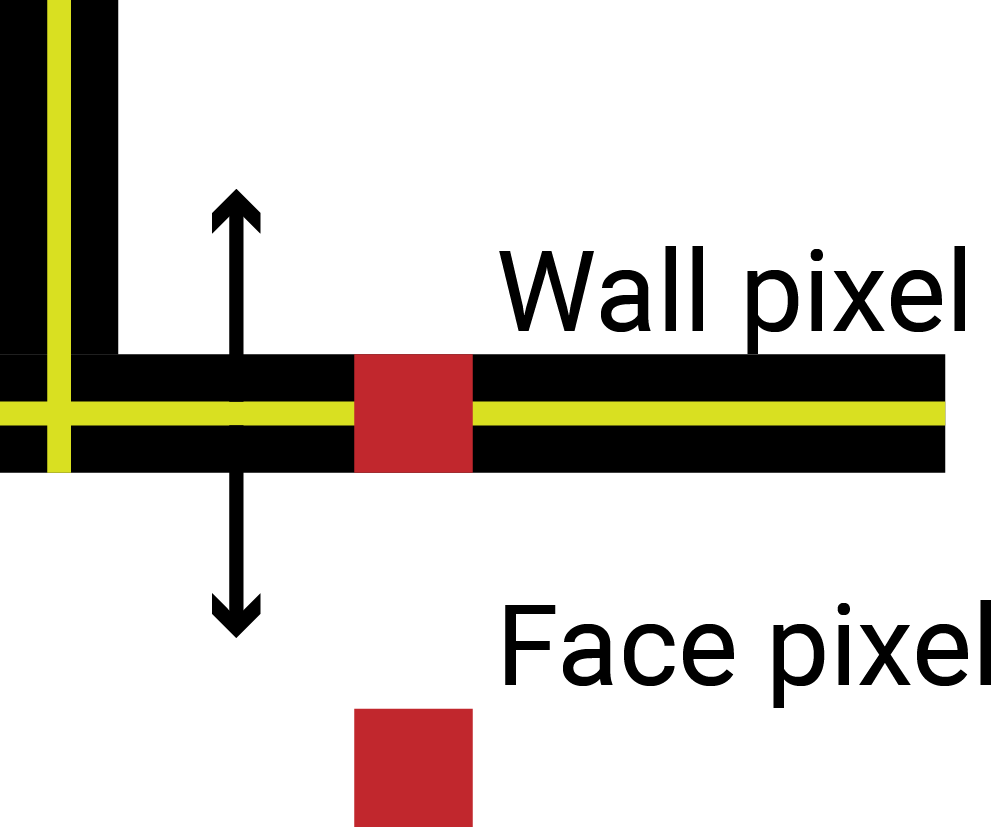
\includegraphics[width=4cm]{images/orientation_computation}
		\caption{Face orientation computation}
		\label{fig:orientation_computation}
	\end{figure}
	
	Because of depth sensor inaccuracy, the computed map pixel coordinate doesn't always lie on the wall. In figure \ref{fig:orientation_computation}, computed face pixel is coloured red. \\
	
	Using a simple breadth first search in face pixel position proximity, the closest wall pixel is determined. In figure \ref{fig:orientation_computation}, this pixel is also coloured red. \\
	
	After wall pixel has been found, the Hough line finding algorithm is applied to an area around wall pixel. The detected lines in figure \ref{fig:orientation_computation} are represented with green colour. If more than one line is found, the line which is closest to the wall pixel is selected. After the line is found, there are two possible orientations as represented in figure \ref{fig:orientation_computation}. The vector that is pointing in the direction of the robot is chosen to be the face orientation. \\
	
	A similar algorithm is used to detect ring orientation.
	
	\subsubsection{Face classification}
	After faces are detected and localized in the world, the faces are identified.
	
	\subsection{Colour classification}
	The robot must be able to detect ring and cylinder colours. There are six possible classes: black, white, red, green, blue and yellow. \\
	
	In homework 2, we tested different colour spaces and classification models and concluded that the k-nearest neighbours algorithm worked best. The colour space with the highest accuracy in homework was \texttt{HSV} colour model, but in the Gazebo simulator, \texttt{RGB} space worked better. \\
	
	So the colour classifier in the final task uses the k-nearest neighbours algorithm and takes in an input vector in $(red, green, blue)$ format and returns a colour label. \\
	
	Because of the non-even lighting in the Gazebo simulator (and probably real world too), the classifier sometimes returns incorrect label. The problem was solved using the robustification process as described in the \ref{robustification} section. Colour classifier is run multiple times on different object detections and the most frequent colour is chosen as the object colour. \\
	
	\subsection{Rings}
	In this section, the algorithm for ring detection is presented.
	
	\subsubsection{Ring detection}	
	\subsubsection{Ring color detection}
	
	\subsection{Cylinder detection}
	\subsubsection{Removal of planes}
	\subsubsection{Cylinder detection}
	\subsubsection{Approaching point computation}
	
	\subsection{Robustification} \label{robustification}
	The sensor data that the robot receives is not always accurate. When object is detected, the depth sensor might have computed the distance inaccurately or the robot was not localized. The detectors might also return false positives and so on. \\
	
	To combat this, a robustification is performed on detected objects. The object detectors are sending detections to robustifier, which collects data and determines if the detection is a true positive or not. \\
	
	For detection to be considered true positive, the following must hold:
	\begin{enumerate}
		\item Detected object should be detected at least \texttt{threshold} times
		\item There must be at least \texttt{minimum distance} meters between this detection and every other previous detection.
	\end{enumerate}

	If two detections are close enough (the distance is less than \texttt{minimum distance}), they are considered the same object. The world position and approaching point position of those two detections are averaged. So the object position is closer to its actual position in space.
	
	\subsection{Smart exploration of space}
	\subsection{Fine movement}
	
	\section{Implementation and integration}
	% Image of our final arhitecture
	
	\section{Results}	
	\section{Division of work}
	% We should only write what each of us did here and add that the professor should compute percentages himself.
	
	\section{Conclusion}	
	
\end{document}